\documentclass[mathserif]{article}
\usepackage{fullpage}
\usepackage{pgffor}
\usepackage{amssymb}
\usepackage{bm}
\usepackage{mathtools}
\usepackage{verbatim}
\usepackage{appendix}
\usepackage{graphicx}
\usepackage{amsmath}
\usepackage[UKenglish]{isodate} % for: \today
\cleanlookdateon                % for: \today
\newcommand\numberthis{\addtocounter{equation}{1}\tag{\theequation}}

\def\wl{\par\vspace{\baselineskip}\noindent}
\def\beginmyfig{\begin{figure}[htbp]\begin{center}}
\def\endmyfig{\end{center}\end{figure}}
\def\prodl#1#2#3{\prod\limits_{#1=#2}^{#3}}
\def\suml#1#2#3{\sum\limits_{#1=#2}^{#3}}
\def\ds{\displaystyle}
\def\tbf#1{\textbf{#1}}
\def\inv{^{\raisebox{.2ex}{$\scriptscriptstyle-1$}}}
\def\pm{^{\raisebox{.2ex}{$\scriptscriptstyle\prime$}}}
\newcommand{\m}[1]{\mathbf{\bm{#1}}} % Serif bold math

\begin{document}
% my title:
\begin{center}
  \section*{\textbf{Predicting Germination Rates of Different Tulip
                    Populations at Various Chilling Times}
    \footnote{https://github.com/luiarthur/Fall2014/tree/master/Stat637/project/tulip}
  }
  \subsection*{\textbf{Arthur Lui}}
  \subsection*{\noindent\today}
\end{center}

\section*{Introduction}
Tulips popularized in the sixteenth century in Holland. During the tulipomania,
a viceroy bulb could allegedly be exchanged for a basket of goods, some
furniture, \textit{and} some live stock. Today, nine million bulbs are produced
annually, and tulips account for 25\% of agricultural exports. Many tourists
also come to the Netherlands to see the vast tulip fields each year. Since
tulips are such a prominent part of the Dutch economy, the country is anxious
about maximizing the growth of these beautiful flowers.\\

\noindent
A major factor that affects the growth of tulips is termed the ``chill time" of
the tulip seeds. Chill time is defined as the time that a (tulip) seed is
present in temperatures below 55$^\circ$F, prior to germinating. If
insufficient chill time is given to tulip seeds, they are not as likely to
germinate and flower. On the other hand, too much chill time can also adversely
affect the germination rates of the seeds.  Most tulips need 12-14 weeks of
chill time. For a given variety of tulip, a population of tulips may exhibit different
responses to chill times due to its conditioning. That is, some tulip populations
may be more robust to adverse weather effects than others. Hence, scientists are
interested in identifying tulip populations that are more resilient so as to 
breed those types of tulips more widely. Specifically, due to global warming, 
scientists want to identify the tulip populations that are able thrive most
in warmer weathers, and require a shorter chill time.\\

\noindent
In order to identify tulip populations that are most resilient to warm weather
climates, we were given a dataset from Dr. Matthew Heaton, containing
information of eleven tulip populations at a research farm in the Netherlands.
Each tulip population was treated with seven chilling times (0,2,4,6,8,10, and
12 weeks). These chilling times were artificially created by placing the tulip
seeds in chillers. For each of the eleven populations, thirty seeds were
observed for each of the seven chilling times. So, a total of 2310 = 30*7*11
observations are contained in this dataset. In the dataset, information on each
of the 2310 tulip seeds is provided. One column indicates weather the seed
germinated (Y/N). Another column indicates the population the seed belongs to
(1-11). And yet another column shows the chill time given for each seed
(0,2,4,6,8,10,12). Two other variables containing the dates the tulip seeds
were harvests were not used for this study. Figure 1 shows the germination
rates over all populations at the 7 different chill times (top left), and
the germination rates for each of the eleven populations at the 7 different
chill times.\\
\beginmyfig
    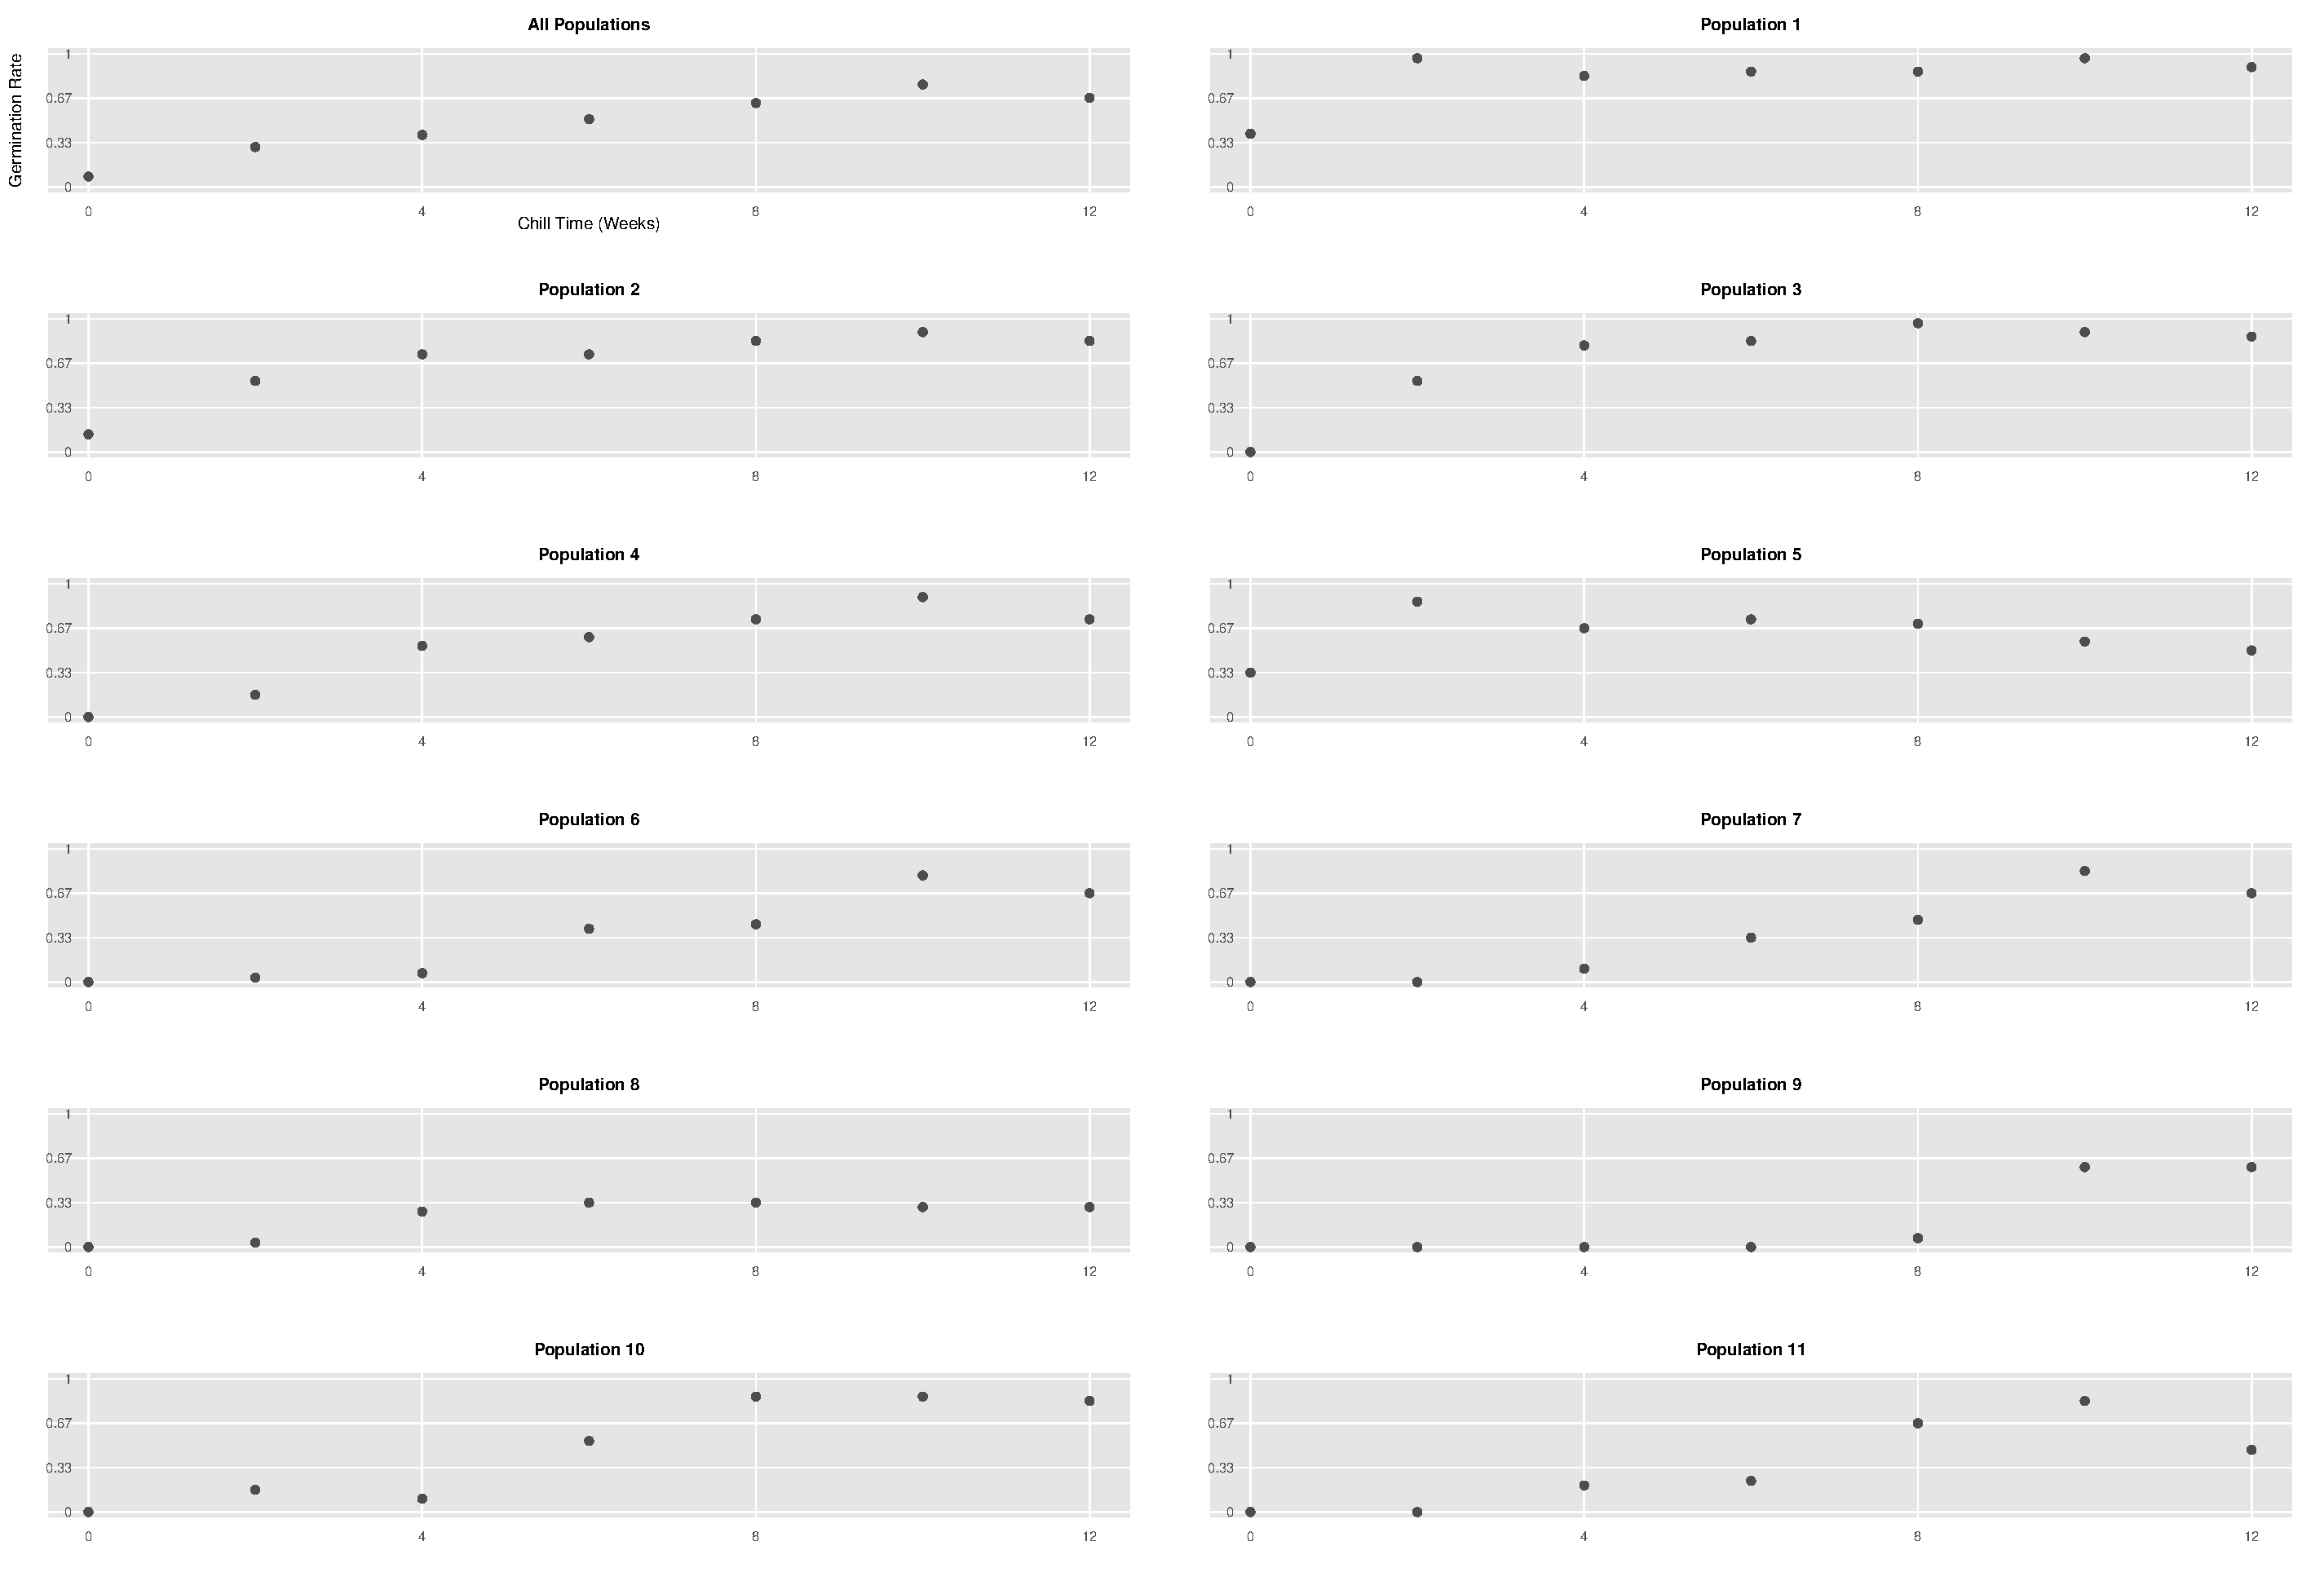
\includegraphics[scale=.35]{../../images/rawData.pdf}
    \caption{Germination rates over all populations at the 7 different
             chill times (top left), and the germination rates for each of 
             the eleven populations at the 7 different chill times.}
\endmyfig

\noindent
For this project, our goal is to identify (1) the effect of chill time for each
tulip population, (2) the optimal chill time for each population, and (3) how
the optimal chill times differ by population. To determine these items, we will
use a Bayesian probit model for our data, with chilling time and population as
our predictors, and whether the seed germinated as our response. We will
introduce the model in the following section, and provide interpretation the
results of our analysis in the next section.\\

\section*{Model}
Since we are modeling (germination) rates, it would be appropriate to use a
logistic regression or a Bayesian probit model. After fitting both models, I
decided to use the Bayesian probit model I decided to use the Bayesian probit
model due to the ease of obtaining interpretable credible intervals. In the 
following subsection, we outline the model definition.\\

\subsection*{Model Definition}
We model $y_i$ with a Bernoulli($p_i$) distribution. And place a probit link on
$p_i$. That is the link function is the inverse cumulative distribution
function of the standard normal distribution. We set the link function to be
the linear combination of the splined covariates $\m{b(x_i)}$ in the design
matrix and the coefficients $\m{\beta}$.  Here, $\m{x_i'}$ is a vector of
length 2, and is (1,$x_i$). We will define $\m{b(x_i')}$ to be a vector of
length 48. The first element is 1. The next three elements are the resulting
values of a basis expansion for a cubic polynomial. We place a cubic polynomial
for our chill times because it is clear from a plot of our empirical data show
in Figure 1 that, in general, germination rates peak at a certain chill time,
but then decrease below and beyond an optimal chill time.  The next 44 elements
are either 0,1, or $b(x_i)$, depending on the tulip population $i$. After
specifying the likelihood, we specify a prior for $\m{\beta}$. We will put a
Normal prior on $\m{\beta}$ centered at 0. Below, we outline the model
definition in mathematical terms.\\
\begin{center}
  \begin{tabular}{rl}
    $y_i  \sim$& \text{Bernoulli}($p_i$)\\
    $\Phi\inv(p_i) =$&$ \m{b(x_i')\beta}$ \\
                  $=$&$ \beta_0 + \suml{j}{1}{3}\beta_j b_j(x_i) +
                        \suml{k}{1}{11} \beta_{0j}\cdot I\{\text{pop}_i=k\} + $\\
                $ $  &$ \suml{k}{1}{11} \suml{j}{1}{3}\beta_{1j}\cdot I\{\text{pop}_i=k\} b_j(x_i)$\\
                 &\\
    \text{Let $\m{W=b(X)}$}, & \\
    $\m{\beta}\sim$&$\text{Normal}\left(\m{0},s_b^2\m{(W\pm W)\inv}\right)$
  \end{tabular}
\end{center}

%\subsection*{Model Diagnostics}
%\subsection*{Model Comparison}
%\subsection*{Model Interpretation / Variable Selection}

%Parameter Interpretation
\section*{Results}
Parameter estimates for the model are shown in Figure 2. The posterior means and
95\% HPD's are included. While some parameters' HPD's include 0, they are still
included in the model as it is not sensible to exclude them while keeping other
terms from the same cubic polynomial. The trace plots are not shown here as
there were 48 of them. But they all appear to indicate that the chain has
converged to the correct distribution.
\beginmyfig
  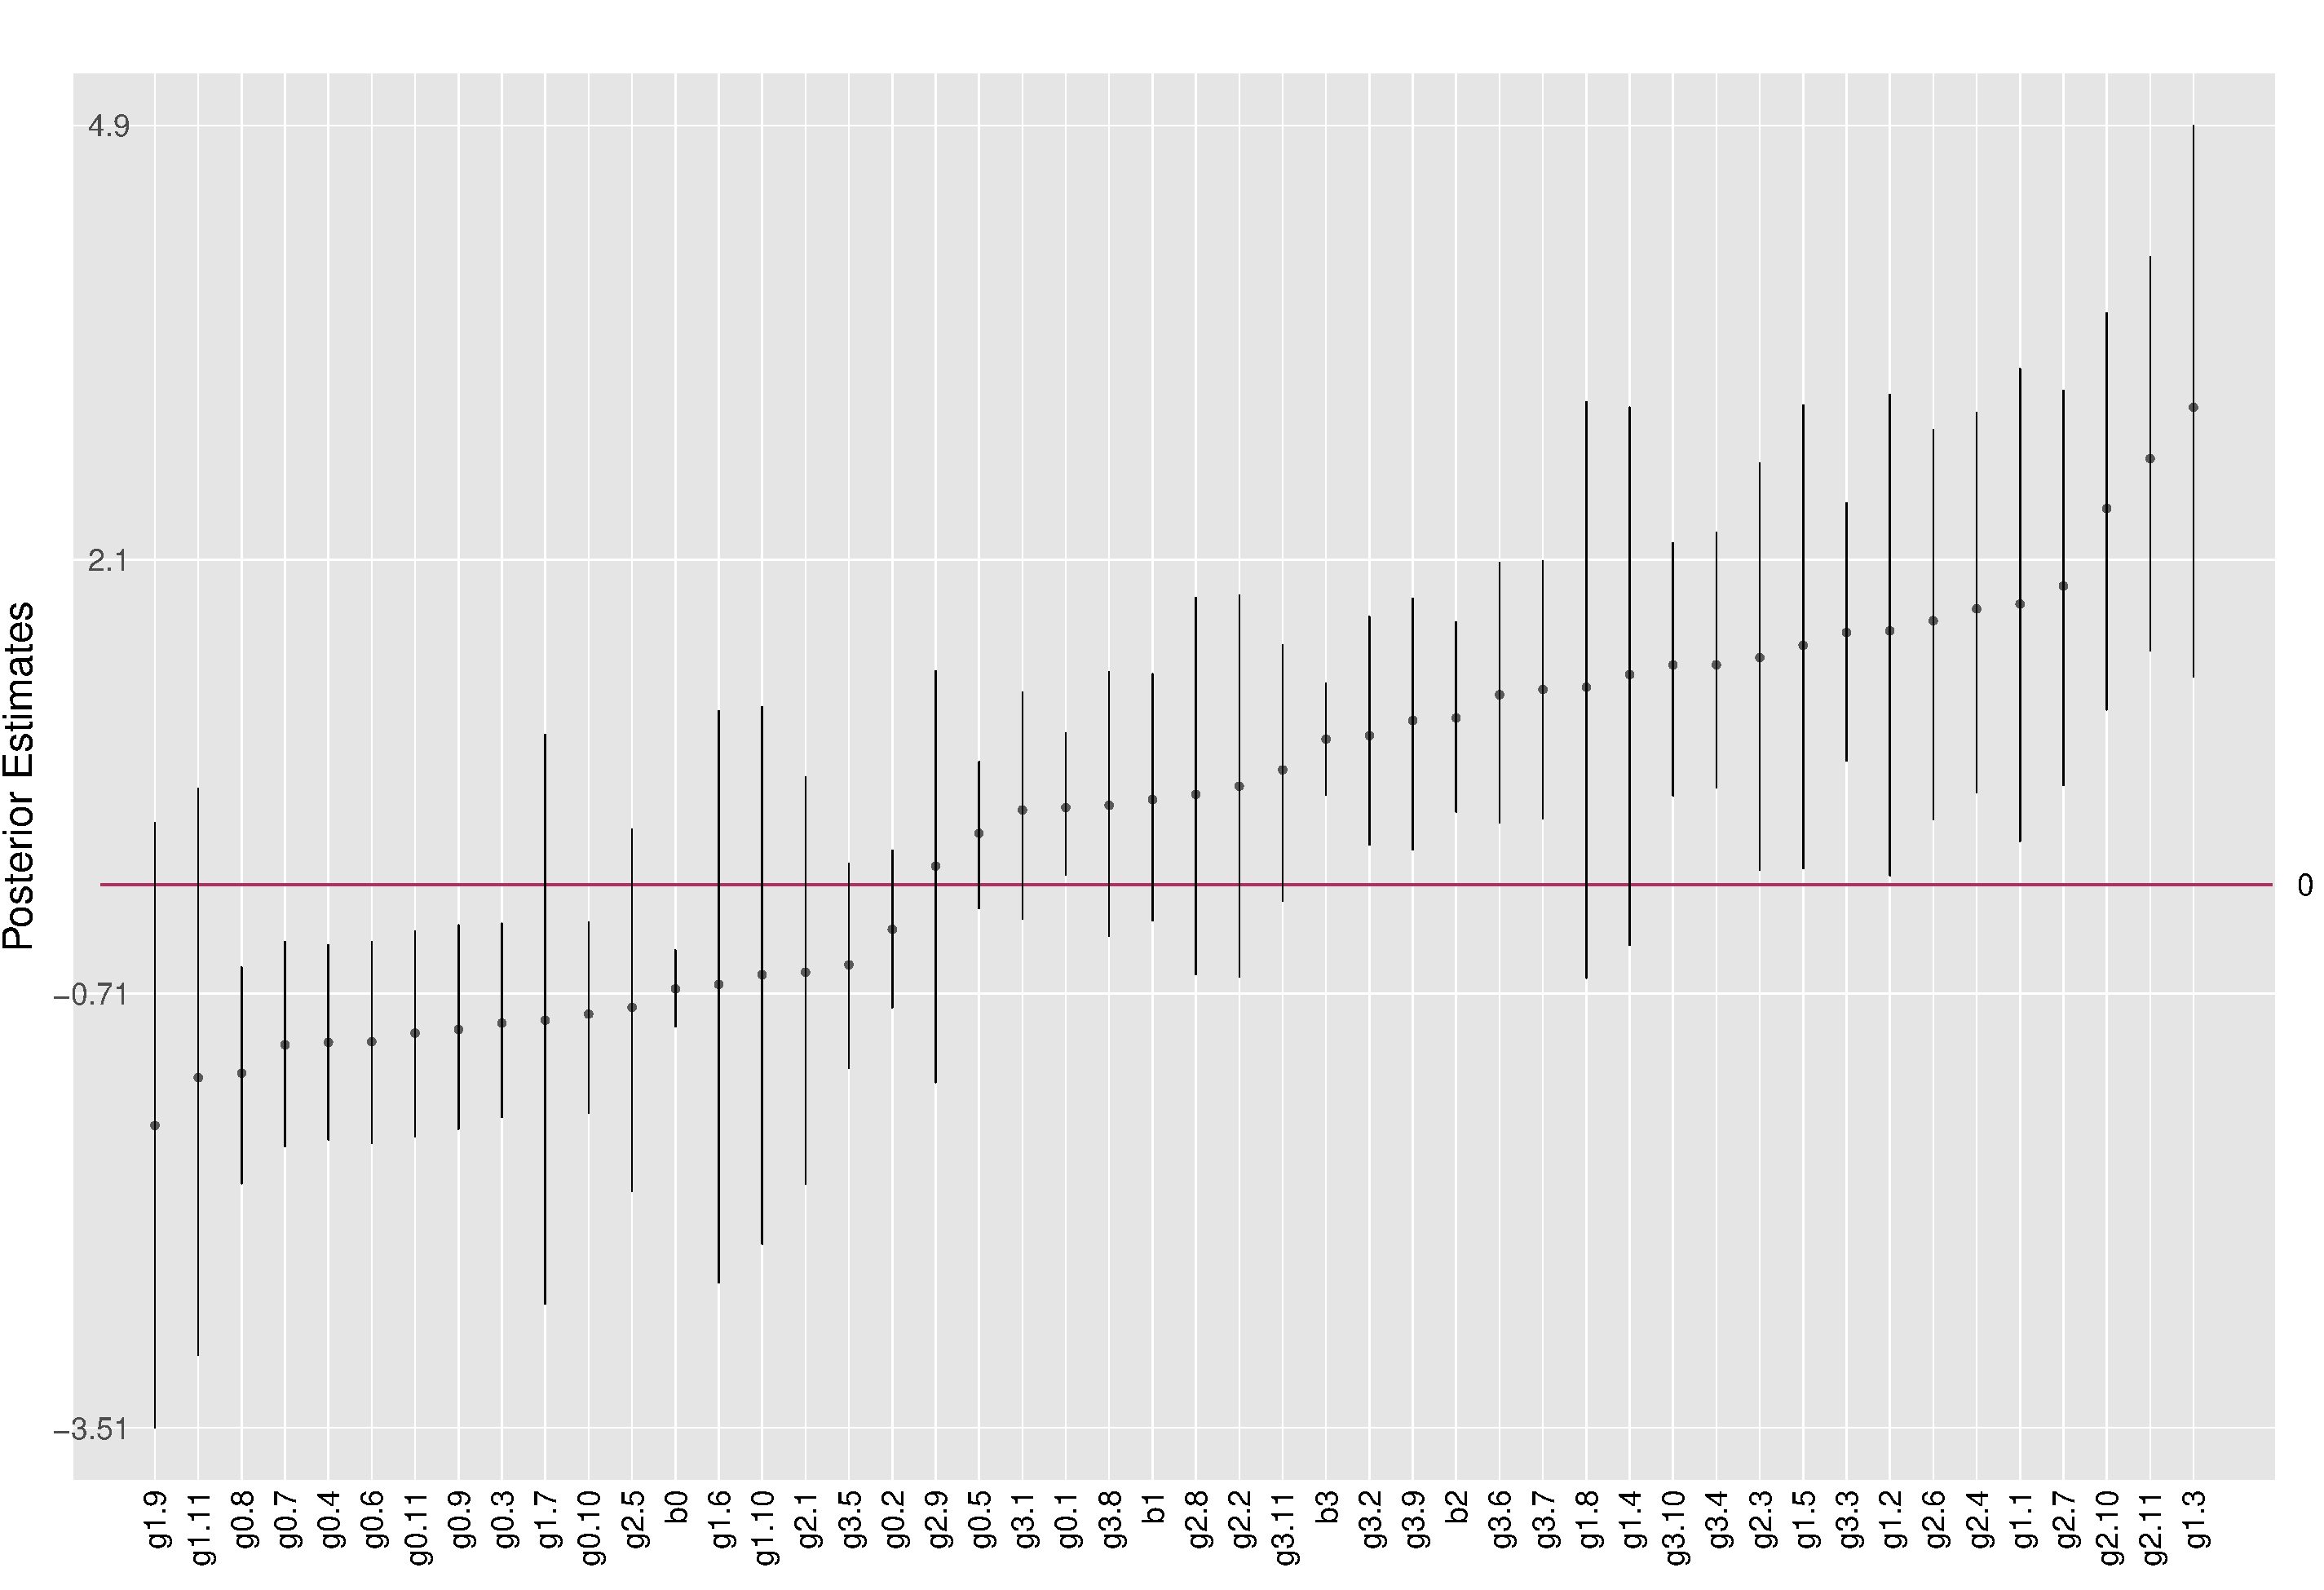
\includegraphics[scale=.35]{../../images/hpd.pdf}
  \caption{Parameter posterior means and 95\% HPD's. While there
           are parameters which HPD's include 0, they are still
           included in the model as it is insensible to
           exclude them while keeping other coefficients from
           the same cubic polynomial.}
\endmyfig  
It is cumbersome to interpret these parameters as we have used a cubic spline.
Instead of address the parameters, we will interpret the posterior predictive
lines over all chill times for each tulip population, show in Figure 3.
\beginmyfig
  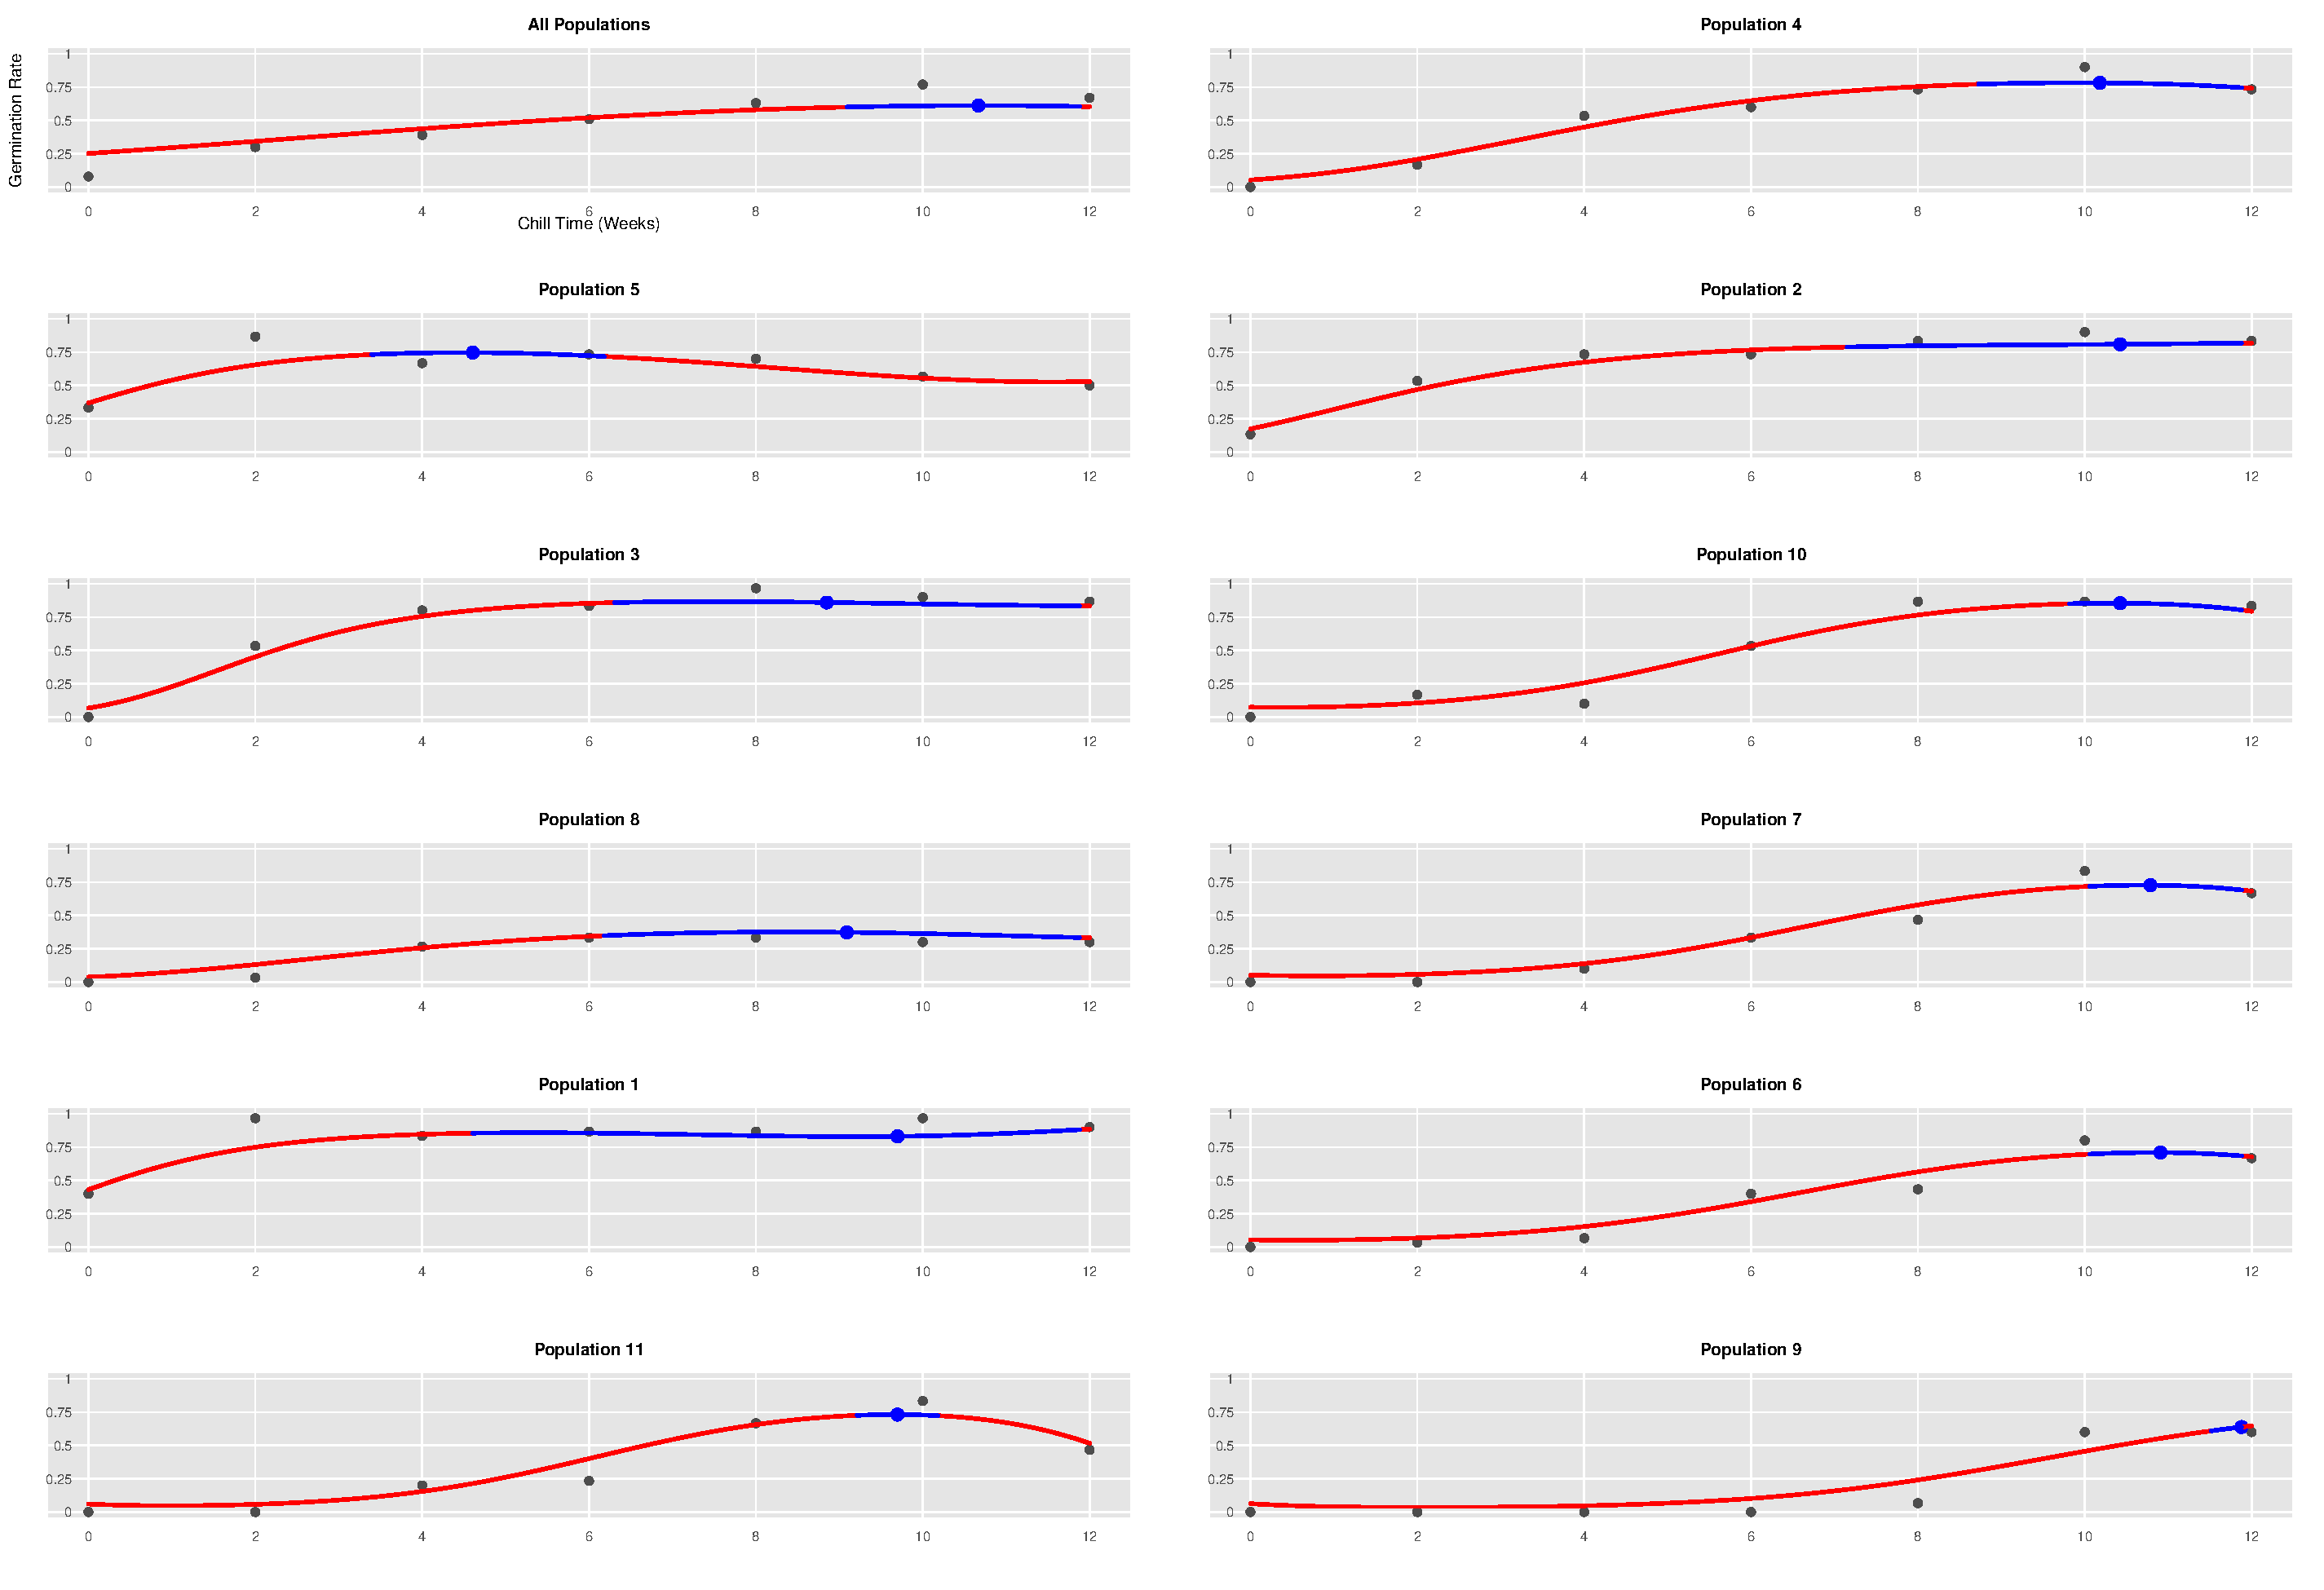
\includegraphics[scale=.35]{../../images/chilleffect.pdf}
  \vspace{-2mm}
  \caption{Predicted germination rates of each population of tulips by
           chilling times (weeks)}
\endmyfig
The top left graph shows the original empirical mean germination rates (grey
dots), with the posterior predictive obtained using the posterior distribution
of the parameters $\beta$ and $\gamma$. The trend of the line suggests that
over all populations, as chilling time increases from 0 weeks to 10.7 weeks,
germination rates increase. But past 10.7 weeks, germination rates decrease as
chilling time increases. The blue point represents the estimated optimal chill
time over all populations, which is 107 weeks. The blue region is the 95\% HPD
for the optimal chill time, which is ranges from 9.5 to 12 weeks. At the
optimal chill time, germination rates over all populations reach 60\%. This is
not the most efficient of germination rates.\\

\noindent
Similar interpretations can be made for individual populations. We will not
discuss each of the populations' optimal chill times, but point out a few
interesting observations. Population 5 has an optimal chill time of 4.3 weeks,
the 95\% HPD covers 3.8 to 6 weeks. We expect that at the 5\% $\alpha$ level,
there would not be able to germinate significantly more tulips by varying the
chill time between 3.8 to 6 weeks. Beyond the HPD, germination rates decrease.
Germination rates for population 5 increase sharpest at the beginning from 0 to
3 weeks, and germination rates decrease at a more gradual pace, beyond 6 weeks.
Population 5 requires the least amount of chill time. At its optimal chill
time, population 5 has a germination rate of 75\%. I think this is rather good.
This yield ranks 6$^{th}$ out of the 11 populations. Populations 3 and 10 have
germination rates of 80\% at their optimal chill times. But they require 4 to 6
weeks more chill time to achieve their optimal yields. This suggests that
in warm weather conditions, population 5 will not only thrive, but yield the
highest germination rates. In this sense, population 5 is very efficient.\\

\noindent
Population 11 appears to have the most well defined optimal chill time. Its HPD
is relatively short, spanning 9.6 and 10.1 weeks. The estimated optimal chill
time is 9.8 for that population. At its peak, it a yields 75\% germination rate.\\

\noindent
Population 9 requires the most amount of chill time. The estimated optimal chill time
is 12 weeks, with a 95\% HPD from 11.9 to 12 weeks. It also appears that
the true optimal chill time for population 9 is greater than 12 weeks.
This indicates that we will need for chill times beyond 12 weeks to make
accurate inference for population 9. Note that it is unclear what the
germination rate will be at the optimal chill time, so it may be the 
case that at its optimal chill time, population 9 will yield far more 
germinated seeds than other populations.\\

\noindent
Populations 3 and 10 have the highest germination rates of 80\% at their optimal chill times,
9 and 10.5 weeks, respectively. However, the HPD for population 3's optimal chill time
spans 6.2 to 11.9 weeks, while the HPD for population 10's optimal chill time spans
9.8 to 11.9 weeks. So, I population 3 is more robust to warm weather conditions
than population 10.\\

\noindent
Population 8 is relatively weak compared to other populations. Even at its optimal chill
time, which is high at 9 weeks, it yields a 30\% germination rate. Compared to population 3,
and population 1, which have similar optimal chill times but over double the germination
rates, it is clear that population 8 is weaker at reproducing and should not be sown as much
so as to reserve natural resources for other populations. Nevertheless, perhaps population
8 may have some other desirable properties, such as pleasant fragrances and more attractive
colors. Further investigation is warranted for this population.\\

\noindent 
For years with shorter winters (with 4-6 weeks of temperatures below 55$^\circ$F), I would
recommend sowing more population 1 and 5 seeds as they can reach their maximum germination rate
\textit{and} yield a high proportion of germinated seeds. For longer winters (10-12 weeks), 
I would recommend sowing more of populations 1,2,3,4,6,7, and 10. For medium-length winters
(6-8 weeks), I would recommend sowing more of populations 1 and 3. Last of all, more investigation
is needed for populations 8 and 9 to learn more about the qualities of population 8 tulips and
see if population 9 yields a higher germination rate at higher chill times.\\


\section*{Conclusion}
Overall, the model fits the data well as the predicted lines follows the 
data closely. Our model has appeared to converge from our trace plots
but have not been included in this report as there are 48 of them. Some
are not significantly different than 0 but are still included in the model
as it is not sensible to remove them when are chill times are turned
into cubic polynomials. As mentioned previously, it would be recommended
to sow certain seeds for winters of various lengths. And further investigation
needs to be conducted for populations 8 and 9 so as to investigate their
characteristics.

\end{document}
